\chapter{\label{chap:theory}Fundamentação Teórica}
Neste capítulo, apresentaremos a base teórica necessária para compreender o
funcionamento das técnicas de inteligência artificial escolhidas para realizar o
desenvolvimento dos agentes inteligentes de \textit{Spelunky}. Nas seções
\ref{section:environment} e \ref{section:agents}, definimos as características
dos ambientes e os tipos de agentes em inteligência artificial. Em seguida, nas
seções \ref{section:machine-learning}, \ref{section:neural-networks} e
\ref{section:evolutionary-algorithms}, descrevemos os conceitos básicos de
aprendizado de máquina, redes neurais artificiais e algoritmos evolutivos,
conteúdos necessários para se ter um entendimento da técnica \textit{NEAT}
(explicada na seção \ref{section:neat}). Depois disso, investigamos a teoria por
trás das \textit{Behavior Trees} outra técnica de inteligência artificial
utilizada para construção de agentes inteligentes.

\todo[inline]{Remover referência para Behavior Trees}

%----------
\section{\label{section:environment}Ambientes}
Todas as percepções e ações executadas por agentes racionais ocorrem no
\textbf{ambiente} no qual ele está inserido. A quantidade e variedade de
ambientes encontrados é vasta, mas é possível identificar dimensões (ou
características) de classificação para realizar uma categorização destes
ambientes. Estas características irão determinar que tipos de agentes --
enumerados na seção \ref{section:agents} -- são apropriados para cada ambiente.
As dimensões utilizadas para categorizar ambientes são:

\begin{description}
	\item[Observável, Parcialmente Observável ou Não-Observável]
		Um ambiente é observável se os sensores do agente lhe permitirem acesso
		completo ao estado do ambiente a cada ponto no tempo, o que torna este
		tipo de ambiente muito conveniente. O ambiente é parcialmente observável
		se os sensores do agente possuirem ruído ou não tiverem acesso completo
		ao ambiente. Se o agente não possuir nenhum tipo de sensor, então o
		ambiente é não-observável.

	\item[Agente Único ou Multi-Agente]
		Quando o agente não precisa interagir com nenhum outro agente no
		ambiente, então trata-se de um ambiente com agente único. Caso ele
		precise interagir de alguma forma (competição, cooperação ou
		comunicação) com outros agentes, então o ambiente é multi-agente.

	\item[Determinístico ou Estocástico]
		Um ambiente é determinístico caso não exista incerteza sobre o estado
		resultante da execução de uma ação em um determinado estado. Se houver
		qualquer grau de incerteza, o ambiente é estocástico.

	\item[Episódico ou Sequencial]
		Em ambientes episódicos, a experiência do agente é dividida em episódios
		atômicos, ou seja, são independentes entre sí. O agente não precisa
		pensar adiante pois, a cada episódio, recebe informações sensoriais e
		executa apenas uma ação, e o próximo episódio não será influenciado pela
		ação anterior. Já em ambientes sequenciais, a ação atual pode
		influenciar todas as decisões futuras, ou seja, ações a curto prazo
		podem ter consequências a longo prazo.

	\item[Discreto ou Contínuo]
		Ambientes discretos são aqueles onde se tem um número contável de ações
		e percepções possíveis. Em ambientes contínuos, o número de ações e de
		percepções muitas vezes são baseados em valores contínuos ou não são
		contáveis.

	\item[Conhecido ou Desconhecido]
		Esta distinção não se refere ao ambiente em sí, e sim sobre o
		conhecimento do agente (ou criador do agente) das ``leis'' de
		comportamento do ambiente. Em um ambiente conhecido, os resultados (ou
		probabilidades de resultados) das ações são conhecidos. Quando o
		ambiente é desconhecido, o agente precisa primeiro aprender como o
		ambiente funciona para saber fazer escolhas boas para atingir seus
		objetivos.
\end{description}


%----------
\section{\label{section:agents}Agentes Racionais}
Um agente é uma entidade que utiliza seus \textbf{sensores} para perceber o
ambiente no qual está inserido e interage através de seus \textbf{atuadores},
direcionando seus esforços para alcançar algum objetivo que se propõe a atingir
\cite[cap. 2]{RussellNorvig200912}. Um exemplo de agente racional é o ser
humano, que percebe o ambiente através de seus sentidos (visão, audição, entre
outros) e executa ações com seu corpo (braços, pernas, etc.). De acordo com
Russell \& Norvig \cite{RussellNorvig200912}, agentes racionais são agrupados
nas seguintes categorias: \textbf{agentes reflexivos}, \textbf{agentes baseados
em modelo}, \textbf{agentes baseados em objetivos} e \textbf{agentes baseados em
utilidade}.

Os \textbf{agentes reflexivos} são programados para executar ações baseadas em
algum evento percebido. Fica evidente que este tipo de agente simplesmente
executa uma ação baseado em suas percepções imediatas e não guardam informações
sobre suas experiências passadas, sendo apenas reativos.

Diferentemente dos agentes reflexivos, \textbf{agentes baseados em modelo} são
capazes de guardar informações sobre suas experiências passadas e sobre seu
estado atual. Este tipo de agente compreende como suas ações modificam o
ambiente onde está inserido e como o ambiente se altera independentemente de
suas ações, efetivamente construíndo um \textbf{modelo} do ambiente. 

As vezes, ter conhecimento sobre o estado atual do ambiente não é suficiente
para decidir que ação executar. O agente precisa de alguma informação de que
situações são desejáveis, ou que objetivos desejar cumprir. Este é o caso de
\textbf{agentes baseados em objetivo}, que combinam um modelo do ambiente com
informações de objetivo para escolher as ações que mais o aproximam dos estados
desejáveis. A escolha de ações baseada em objetivos pode ser simples -- quando,
por exemplo, o objetivo é antigido com a execução de apenas uma ação -- ou
complexo -- quando, por exemplo, o agente deve considerar longas cadeias de
ações para atingir seus objetivos.

Em alguns casos, os objetivos não são suficientes para gerar comportamentos de
alta qualidade. Por exemplo, muitas vezes é possível atingir um objetivo através
de várias sequências de ações, mas algumas sequências são mais rápidas, mais
seguras, mais confiáveis ou mais baratas. Os \textbf{agentes baseados em
utilidade} fazem uso de uma função de utilidade para medir sua performance e,
assim, distinguir estados mais desejáveis e menos desejáveis. O agente, então, é
capaz de escolher as ações mais vantajosas para ele, aumentando sua performance.


%----------
\section{\label{section:machine-learning}Aprendizado de Máquina}
Quando queremos resolver um problema através de um programa de computador,
desenvolvemos um algoritmo que, dado uma entrada, executa uma sequência de
operações para fornecer uma resposta adequada para a tarefa em questão. Um
exemplo disso são os algoritmos para ordenação de números, onde a entrada é
um conjunto de números e a resposta é o conjunto ordenado. Para alguns
problemas, contudo, nem sempre é possível se chegar a um algoritmo que resolve
satisfatóriamente uma tarefa. Por exemplo, a tarefa de diferenciar
\textit{e-mails} de \textit{spam} e \textit{e-mails} legítimos é complexa, pois
os \textit{e-mails} de \textit{spam} estão mudando constantemente, e a
categorização de \textit{spam} pode variar de indivíduo para indivíduo. Assim,
criar manualmente um algoritmo para resolver esta tarefa pode ser extremamente
complexo ou até mesmo impraticável. A partir deste contexto, surgiu a área de
\textbf{aprendizado de máquina}, que estuda algoritmos que fornecem a programas
de computador a habilidade de aprender e se aperfeiçoarem, tornando-os capazes
de resolver tarefas sem serem explicitamente programados.

Existem três tipos principais de aprendizado de máquina \cite[cap.
18]{RussellNorvig200912}, que são diferenciados entre sí pela natureza dos dados
utilizados para aprender. Estas categorias são: \textbf{aprendizado
supervisionado}, \textbf{aprendizado não-supervisionado} e \textbf{aprendizado
por reforço}. No aprendizado supervisionado, é fornecido um conjunto de dados
com exemplos de entrada e resultados esperados para aquelas entradas. Assim, a
tarefa neste tipo de aprendizado consiste em aprender uma função que mapeia
entradas para saídas. No aprendizado não-supervisionado, o programa recebe um
conjunto de dados de entrada mas não recebe informações com o tipo de saída
esperado. O objetivo deste tipo de aprendizado geralmente é detectar padrões em
conjuntos de dados.  O último tipo de aprendizado, o aprendizado por reforço, é
diferente dos demais porque está diretamente ligado ao conceito de agentes
racionais.  Neste tipo de aprendizado, o agente interage com um ambiente
dinâmico e deve atingir algum objetivo. Quando o agente executa ações no
ambiente, é fornecido a ele algum tipo de retorno -- recompensas ou punições --,
para que ele possa aprender a agir da maneira correta a fim de atingir seus
objetivos.

Para agentes racionais, a capacidade de aprender fornece a oportunidade de se
tornar mais competente que o permitido pelo seu conhecimento inicial do problema
e do ambiente. Problemas como informação incompleta ou inexistente sobre o
ambiente são mais facilmente contornados, pois o agente será capaz de criar um
modelo de representação através do retorno obtido após a execução de ações.


%----------
\section{\label{section:neural-networks}Redes Neurais Artificiais}
Uma \textbf{rede neural artificial} é um modelo matemático que busca replicar
computacionalmente (através de aproximações de funções) as capacidades de
processamento de informações de sistemas nervosos biológicos \cite[Cap.
1]{Rojas:1996:NNS:235222}. É uma técnica de aprendizado de máquina que
recentemente vem recebendo uma atenção especial, mas que teve suas origens no
início da década de 40 \cite[Cap. 18]{RussellNorvig200912}. Esta seção apresenta
apenas um resumo geral de redes neurais artificiais, pois o assunto é muito
complexo e um entendimento superficial do funcionamento desta técnica é
suficiente para este trabalho.

Os elementos fundamentais das redes neurais artificiais são as unidades de
processamento chamadas \textbf{neurônios} (também conhecidas como
\textit{perceptrons}) -- ilustrado na Figura \ref{fig:neural-networks-neurons}
\cite[Cap. 3]{Rojas:1996:NNS:235222}.  Cada neurônio possui um ou mais
\textbf{canais de entrada}, uma \textbf{função de integração}, uma
\textbf{função de ativação} e um ou mais \textbf{canais de saída}. O
funcionamento de um neurônio se dá da seguinte maneira: primeiro, a unidade
recebe as informações que deverá processar através de seus canais de entrada.
Estes canais possuem um \textbf{peso} atrelado a eles, que informa à unidade o
quão importante é a informação advinda daquela conexão. A origem das informações
não é relevante para o neurônio, e podem vir de outros neurônios ou de outras
classes de unidades de processamento (como a entrada da rede, por exemplo).
Todas as informações que o neurônio recebe passam por sua função de integração
(que geralmente é uma função de adição), cujo propósito é reduzir o número de
informações para apenas uma.  Depois de integrar as informações, o neurônio
realiza um processamento interno através de sua função de ativação,
transformando as informações recebidas em outro tipo de informação. Esta função
de ativação deve ser escolhida pelo desenvolvedor da rede e geralmente é ou uma
função de limiar (resultado $0$ ou $1$) ou uma função de logística (resultados
em números reais, como a função \textit{Sigmóide}). Na última etapa, o neurônio
envia, através de seus canais de saída, a informação que acabou de processar. Os
canais de saída se ligam com outros neurônios ou com a saída da rede.

% AIMA: page 728, figure 18.19
\begin{figure}[H]
\centering
\begin{tikzpicture}
    \def\layersep{4cm}
    \def\textsep{1.5cm}

    \node (a0) at (0, 2) {$a_0$};
    \node (a1) at (0, 1) {$a_1$};
    \node (an) at (0, 0) {$a_n$};

    \node [xshift=-.3cm, minimum width=\textsep, text centered] at (\layersep, 1) (neuron1) {$\sum_{}^{e_j}$};
    \node [minimum width=\textsep, text centered] at (\layersep + \textsep, 1) (neuron2) {};
    \node [xshift=.3cm, minimum width=\textsep, text centered, font=\footnotesize] at (\layersep + \textsep * 2, 1) (neuron3) {$a_j$};

    \node [font=\footnotesize] at (\layersep + \textsep, 1.5) {g};

    \draw [thick]
        (\layersep + \textsep - .5cm, .5)
            ..
               controls (\layersep + \textsep + .8, .5) and
                        (\layersep + \textsep + .4, 1.5)
            ..
        (\layersep + \textsep + .5cm, 1.5)
    ;

    \node (s0) at (\layersep * 2 + \textsep * 2, 2) {$s_0$};
    \node (s1) at (\layersep * 2 + \textsep * 2, 1) {$s_1$};
    \node (sn) at (\layersep * 2 + \textsep * 2, 0) {$s_n$};

    \node (p0) at (1, 2) {$p_0$};
    \node (p1) at (1, 1.2) {$p_1$};
    \node (pn) at (1, .4) {$p_n$};

    \node (neuron) [shape=ellipse, draw, thick, inner xsep=-.5cm, inner ysep=.5cm, fit={(neuron1) (neuron2) (neuron3)}] {};

    \draw [thick] (neuron.130) -- (neuron.230);
    \draw [thick] (neuron.50) -- (neuron.310);

    \node [text width=\textsep, font=\scriptsize, text centered]
        at (.5, -1)
        {Canais de Entrada}
    ;
    \node [xshift=-.3cm, text width=\textsep, font=\scriptsize, text centered]
        at (\layersep, -1)
        {Função de Integração}
    ;

    \node [text width=\textsep, font=\scriptsize, text centered]
        at (\layersep + \textsep, -1)
        {Função de Ativação}
    ;

    \node [xshift=.3cm, text width=\textsep, font=\scriptsize, text centered]
        at (\layersep + \textsep * 2, -1)
        {Saída}
    ;

    \node [text width=\textsep, font=\scriptsize, text centered]
        at (\layersep * 2.5, -1)
        {Canais de Saída}
    ;

    \path[->,>=latex] (a0) edge (neuron);
    \path[->,>=latex] (a1) edge (neuron);
    \path[->,>=latex] (an) edge (neuron);

    \path[->,>=latex] (neuron) edge (s0);
    \path[->,>=latex] (neuron) edge (s1);
    \path[->,>=latex] (neuron) edge (sn);
\end{tikzpicture}
\caption {\label{fig:neural-networks-neurons}Ilustração que indica os principais
componentes de um neurônio de uma rede neural artificial.}
\end{figure}

Com as unidades de processamento definidas, o próximo passo é entender como elas
se conectam entre sí para formar a \textbf{topologia} da rede neural. Existem,
fundamentalmente, dois modelos básicos de topologia: sem realimentação
(\textit{feed-forward}) e recorrentes \cite[Cap. 18]{RussellNorvig200912}. As
redes sem realimentação, como o próprio nome sugere, possui conexões em somente
um sentido (para frente), ou seja, os neurônios processam as informações apenas
uma vez. Já nas redes recorrentes, um neurônio pode processar informações mais
de uma vez (realimentação de informações processadas anteriormentes pela rede).
Por fins de simplificação, a explicação desta seção se concentrará em redes sem
realimentação.

As redes neurais artificiais sem realimentação geralmente estão estruturadas em
\textbf{camadas}, sendo que os neurônios recebem entradas somente de unidades de
processamento da camada anterior. A topologia da rede é dividida,
essencialmente, em uma \textbf{camada de entrada}, zero ou mais \textbf{camadas
escondidas} e uma \textbf{camada de saída}. Quando a rede não possui camadas
escondidas, ela é chamada de \textbf{camada-única}, e quando possui camadas
escondidas é chamada de \textbf{multi-camada}. Quase sempre é necessário
adicionar camadas escondidas, pois a maioria das funções não podem ser
aproximadas corretamente com apenas uma camada (a função lógica \textit{XOR} é
um exemplo disso). Isto ocorre porque quando se tem apenas uma camada de
processamento, só é possível aproximar funções linearmente separáveis(detalhes
em \cite[Cap. 18]{RussellNorvig200912}). As unidades de processamento são
conectadas (geralmente, todos os neurônios de uma camada possuem conexão com
todos os neurônios da camada seguinte) e a rede neural se forma. Dependendo do
problema, a escolha de quantas camadas e unidades de processamento afeta a
qualidade dos resultados obtidos. Não existe uma ciência exata para definir
quantidades de camadas e neurônios, ficando a critério do desenvolvedor a
análise do problema e a experimentação de topologias \cite[Cap.
18]{RussellNorvig200912}. A Figura \ref{fig:neural-networks-example} ilustra uma
possível topologia de uma rede neural artificial sem realimentação.

% Neural Networks: A Systematic Introduction, page 126, figure 6.1
\begin{figure}[H]
\centering
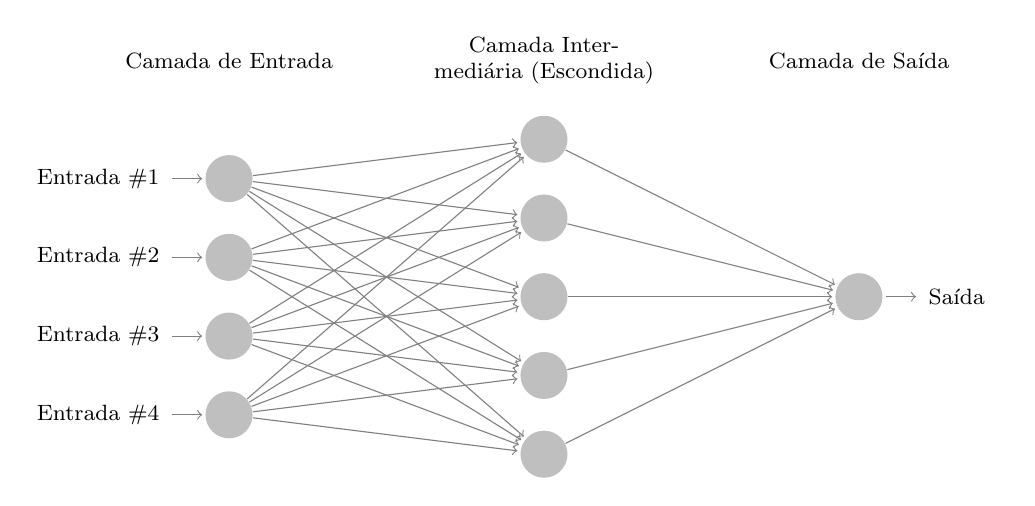
\begin{tikzpicture}[shorten >=1pt,->,draw=black!50, node distance=\layersep]
    \def\layersep{4cm}
    \tikzstyle{every node}=[font=\footnotesize]
    \tikzstyle{every pin edge}=[<-,shorten <=1pt]
    \tikzstyle{neuron}=[circle,fill=black!25,minimum size=17pt,inner sep=0pt]
    \tikzstyle{input neuron}=[neuron, fill=gray!50];
    \tikzstyle{output neuron}=[neuron, fill=gray!50];
    \tikzstyle{hidden neuron}=[neuron, fill=gray!50];
    \tikzstyle{annot} = [text width=10em, text centered]

    % Draw the input layer nodes
    \foreach \name / \y in {1,...,4}
    % This is the same as writing \foreach \name / \y in {1/1,2/2,3/3,4/4}
        \node[input neuron, pin=left:Entrada \#\y] (I-\name) at (0,-\y) {};

    % Draw the hidden layer nodes
    \foreach \name / \y in {1,...,5}
        \path[yshift=0.5cm]
            node[hidden neuron] (H-\name) at (\layersep,-\y cm) {};

    % Draw the output layer node
    \node[output neuron,pin={[pin edge={->}]right:Saída}, right of=H-3] (O) {};

    % Connect every node in the input layer with every node in the
    % hidden layer.
    \foreach \source in {1,...,4}
        \foreach \dest in {1,...,5}
            \path (I-\source) edge (H-\dest);

    % Connect every node in the hidden layer with the output layer
    \foreach \source in {1,...,5}
        \path (H-\source) edge (O);

    % Annotate the layers
    \node[annot,above of=H-1, node distance=1cm] (hl) {Camada Intermediária (Escondida)};
    \node[annot,left of=hl] {Camada de Entrada};
    \node[annot,right of=hl] {Camada de Saída};
\end{tikzpicture}
\caption {\label{fig:neural-networks-example}Ilustração de uma possível topologia
de uma rede neural artificial sem realimentação.}
\end{figure}


O objetivo das redes neurais artificiais, então, é gerar uma \textbf{função de
rede}, que recebe informações na camada de entrada, realiza processamentos com
seus neurônios e envia informações através de um ou mais neurônios na camada de
saída. Esta função de rede deve ser uma aproximação (pois nem sempre atinge
100\% de precisão) da função que queremos descobrir. A rede neural deve passar,
portanto, por um processo de \textbf{treinamento}, que tentará ajustar os pesos
das conexões dos neurônios até encontrar valores adequados. Aqui, o tipo de
treinamento que a rede recebe depende do tipo de aprendizado que está sendo
empregado (supervisionado, não-supervisionado ou por reforço). Um exemplo de
algoritmo de treinamento é o da \textbf{retropropagação}
(\textit{backpropagation}), muito utilizado para treinar redes neurais
artificiais em aprendizado supervisionado. Este algoritmo tenta ajustar os pesos
das conexões através da análise e minimização do erro entre os resultados
esperados (dados de treinamento) e os resultados obtidos através do uso da
função aproximada da rede neural \cite[Cap. 7]{Rojas:1996:NNS:235222}.


%----------
% gene
% genotype
% genome
% phenotype
% individual
% population
% environment
% fitness
% reproduction
% offspring
% mutation
% generation
\section{\label{section:evolutionary-algorithms}Algoritmos Evolutivos}
A \textbf{computação evolutiva} é uma área da Ciência da Computação que, como o
nome sugere, se inspira na ciência da genética e no processo de evolução
natural descrito por Charles Darwin para construir algoritmos que solucionam
problemas computacionais \cite[Cap. 2]{IntroEvolComputing}. Todos os seres
vivos, ou \textbf{indivíduos}, são formados por um \textbf{fenótipo} e um
\textbf{genótipo}. O fenótipo são as características observáveis do indivíduo,
como seu comportamento e seu aspecto físico. Já o genótipo representa a
constituição genética do indivíduo e é descrito por seus \textbf{genes},
unidades funcionais de herança genética presentes dentro de seu \textbf{genoma}
(informação genética completa de um indivíduo). 

O processo biológico de evolução pode ser resumido da seguinte forma: os
indivíduos fazem parte de uma \textbf{população} e vivem dentro de um ambiente.
Como este ambiente possui recursos limitados, a competição por recursos é
natural, e a \textbf{aptidão} de um indivíduo afeta a sua probabilidade de
sobrevivência. Esta aptidão é determinada por seu fenótipo, ou seja, por suas
características físicas e pela maneira na qual interage com o ambiente e os
demais indivíduos. Desta forma, o processo de seleção natural tende a favorecer
indivíduos com boas características fenotípicas.  Quando um indivíduo entra em
processo de \textbf{reprodução}, ele gera \textbf{descendentes}. O genoma dos
descendentes, contudo, não é o mesmo que o de seus pais, pois pequenas variações
genéticas ocorrem durante a reprodução. Desta forma, variações genotípicas são
criadas, que são traduzidas para variações fenotípicas. 

Os \textbf{algoritmos evolutivos} se baseiam neste processo biológico para
resolver problemas computacionais. Para que se possa utilizar um algoritmo
evolutivo a fim de resolver um problema computacional, é necessário espeficiar
uma série de componentes, procedimentos e operadores que definirão seu
funcionamento \cite[Cap. 3]{IntroEvolComputing}. Os componentes mais importantes
são:

\begin{itemize}
	\item Representação (definição dos indivíduos)
	\item Função de aptidão
	\item População
	\item Mecanismos de seleção de pais
	\item Operadores de variação (mutação e recombinação)
	\item Mecanismo de seleção de sobreviventes (substituição de indivíduos)
\end{itemize}

O primeiro passo para definir um algoritmo genético é estabelecer uma forma de
conexão entre o contexto do problema original e o espaço de resolução de
problemas onde a evolução irá atuar. Esta \textbf{representacão} define o
mapeamento entre os fenótipos (possíveis soluções dentro do contexto do
problema) e os genótipos (codificação das soluções dentro do espaço de
resolução). O processo de mapeamento de fenótipo para genótipo é chamado de
\textbf{codificação}, e o processo de mapeamento de genótipo para fenótipo é
chamado de \textbf{decodificação}.

O propósito de uma \textbf{função de apditão} é representar os requisitos que a
população de indivíduos deve respeitar e se adaptar para sobreviver. Geralmente,
a função de aptidão é uma função ou procedimento que fornece uma medida
quantitativa para a performance dos indivíduos.

A \textbf{população} é responsável por armazenar um conjunto de genótipos de
indivíduos a serem testados, e forma a unidade central onde ocorre a evolução.
Dada uma representação, a definição de uma população pode conter a quantidade de
indivíduos, uma função de distância entre indivíduos (para dividí-los em
espécies), entre outros. Em quase todos os algoritmos evolutivos, o tamanho da
população é constante e não aumenta durante o tempo de execução. Isto ajuda a
criar um cenário de recursos finitos e competitividade. 

O papel dos \textbf{mecanismos de seleção de pais} é fazer uma distinção entre
os indivíduos baseados em suas aptidões e permitir que os indivíduos mais aptos
se tornem os pais da próxima geração. Um indivíduo é classificado como um
\textbf{pai} se foi escolhido para sofrer variações e criar
\textbf{descendentes}. A escolha de pais geralmente é probabilística, e os
indivíduos mais aptos possuem mais chances de se tornar pais.

Os \textbf{operadores de variação} são responsáveis por criar novos indivíduos
baseados no código genético de outros indivíduos. Existem dois operadores de
variação: a \textbf{mutação} e a \textbf{recombinação}. A mutação é aplicada em
um genótipo e a recombinação é aplicada em dois genótipos e ambos criam uma
versão levemente modificada dos genótipos utilizados. Estes operadores são
estocásticos, ou seja, a escolha de quais partes dos genótipos serão modificadas
é aleatória.

De maneira similar, o papel do \textbf{mecanismo de seleção de sobreviventes} é
distinguir indivíduos baseados em suas aptidões. Contudo, este mecanismo é
aplicado em outra etapa do ciclo evolucionário. Como a população dos algoritmos
evolutivos é quase sempre constante, é necessário selecionar quais indivíduos
irão para a próxima geração. Esta decisão geralmente é baseada nos valores de
aptidão, favorecendo os indivíduos de maior qualidade, mas também pode ser
baseado na idade dos indivíduos (quanto tempo estão na população). Em contraste
ao mecanismo de seleção de pais, a seleção de sobreviventes é quase sempre
determinístico.

Além de especificar estes componentes básicos, é necessário definir um
procedimento de \textbf{inicialização} e uma ou mais \textbf{condições de
parada}. O procedimento de inicialização é responsável por criar a população
inicial, e a maioria dos algoritmos evolutivos criam uma população inicial
composta por indivíduos gerados aleatóriamente. Existem dois casos possíveis de
parada de um algoritmo evolutivo. Se o valor ótimo de aptidão do problema é
conhecido, a condição de parada ideal é a descoberta de uma solução com esta
aptidão. Contudo, algoritmos genéticos contém muitos elementos estocásticos e,
portanto, nunca se tem garantia total de que a condição de parada ideal será
atingida. Portanto, é necessário extender esta condição de parada para que ela
com certeza seja atingida. As opções mais comuns são limitar o tempo de
execução, o número de iterações, o número de avaliações de aptidão, entre
outros. O algoritmo \ref{alg:evolutionary-algorithm-skeleton} exemplifica o
esqueleto de um ciclo de execução de um algoritmo evolutivo.

\begin{algorithm}[h]
\begin{center}
	\begin{algorithmic}[1]
        \STATE{POPULAÇÃO $\gets$ candidatos gerados aleatóriamente}
		\STATE{AVALIAR cada candidato}
		\REPEAT
			\STATE{SELECIONAR pais adequados}
			\STATE{RECOMBINAR genomas dos pais}
			\STATE{MUTACIONAR os descendentes}
			\STATE{AVALIAR cada novo candidato}
			\STATE{SELECIONAR indivíduos para a próxima geração}
		\UNTIL{CRITÉRIO DE PARADA ATINGIDO}
    \end{algorithmic}
\end{center}
\caption{Ciclo de execução de um algoritmo evolutivo.}
\label{alg:evolutionary-algorithm-skeleton}
\end{algorithm}

A construção de algoritmos que fornecem soluções ótimas para qualquer problema
computacional nem sempre é possível. Por exemplo, o número de possíveis soluções
para um determinado problema pode crescer exponencialmente de acordo com o
número de variáveis consideradas, o que pode impedir seu tratamento em um tempo
aceitável. Portanto, apesar do constante crescimento de poder computacional, a
partir de certo ponto é preciso abandonar a busca por soluções ótimas e
encontrar outros métodos para encontrar soluções boas o suficiente. Os
algoritmos evolutivos são técnicas de \textbf{otimização de função} baseados em
\textbf{heurísticas} cujo objetivo é encontrar a \textbf{máxima local} dentro de
um espaço de estados \cite[Cap. 3]{IntroEvolComputing}. Os indivíduos da
populacão representam tentativas de encontrar a solução ótima para a função, e a
busca local dentro do espaço de estados é auxiliada pelos valores de aptidão e
pelas operações de mutação e recombinação.

Para exemplificar o funcionamento de um algoritmo evolucionário, o cenário
hipotético de maximizar uma função objetiva unidimensional foi criado. A Figura
\ref{fig:evolutionary-algorithms-function} ilustra a distribuição dos indivíduos
da população em três estágios de execução de busca evolutiva. Em um primeiro
momento, logo após a inicialização, os indivíduos estão espalhados
aleatóriamente no espaço de busca
(\ref{fig:evolutionary-algorithms-function-start}). Depois de algumas gerações,
a distribuição muda: graças ao mecanismo de seleção e aos operadores de
variação, a população abandona as regiões que oferecem baixa aptidão
(\ref{fig:evolutionary-algorithms-function-middle}). Ainda depois, toda a
população está concentrada em alguns picos de aptidão, mesmo que subóptimos
(\ref{fig:evolutionary-algorithms-function-end}). A princípio, é possível que a
população escale a colina errada, deixando todos os indivíduos posicionados
próximos de uma máxima local, e não uma máxima global. É necessário que haja um
equilíbrio entre \textit{exploration}, a geração de novos indivíduos em regiões
ainda não testadas do espaço de estados, e \textit{exploitation}, a concentração
da busca em regiões de boas soluções conhecidas.

\begin{figure}[htb!]
\centering
	\begin{subfigure}[b]{0.3\textwidth}
		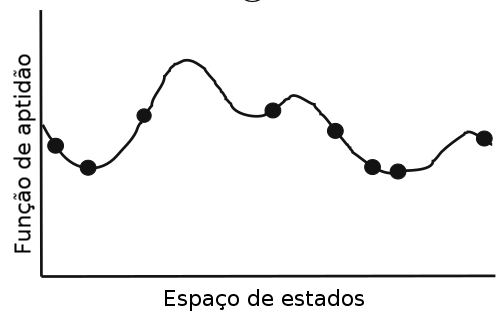
\includegraphics[width=\textwidth]{fig/evolutionary-algorithms-function-start.png}
		\caption{Início}
		\label{fig:evolutionary-algorithms-function-start}
	\end{subfigure}
	\begin{subfigure}[b]{0.3\textwidth}
		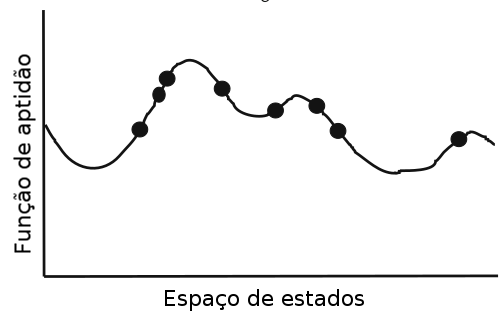
\includegraphics[width=\textwidth]{fig/evolutionary-algorithms-function-middle.png}
		\caption{Meio}
		\label{fig:evolutionary-algorithms-function-middle}
	\end{subfigure}
	\begin{subfigure}[b]{0.3\textwidth}
		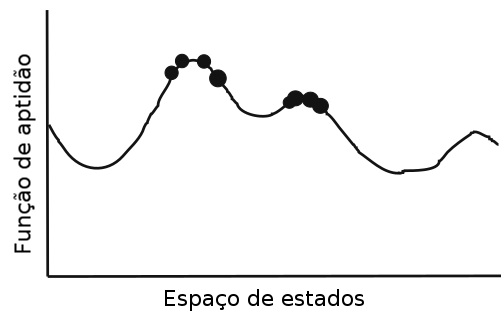
\includegraphics[width=\textwidth]{fig/evolutionary-algorithms-function-end.png}
		\caption{Fim}
		\label{fig:evolutionary-algorithms-function-end}
	\end{subfigure}
	\caption{Exemplo do funcionamento de um algoritmo evolucionário para
	maximizar uma função. O eixo $x$ corresponde ao espaço de busca, o eixo $y$
	mostra o valor de aptidão correspondente e os pontos representam os
	indivíduos da populacão.}
	\label{fig:evolutionary-algorithms-function}
\end{figure}


%----------
\section{\label{section:neat}NEAT}
A \textbf{neuroevolução} é uma forma de aprendizado de máquina que utiliza
algoritmos evolutivos para criar e treinar redes neurais artificiais \cite[Cap.
4]{HandbookNeuroevolution}. Como a neuroevolução busca por um
\textbf{comportamento} ao invés de uma função de valor para cada estado, é muito
eficaz para problemas com espaços de estados contínuos e altamente dimensionais.
Este conceito é muito utilizado para resolver problemas de otimização em
inteligência artificial e em jogos digitais \cite{DBLP:journals/corr/RisiT14}.
Existem dois elementos que podem ser evoluídos em uma rede neural artificial: os
\textbf{pesos das conexões} e a \textbf{topologia}. Quando ambos são evoluídos,
as redes são chamadas de \textit{Topology and Weight Evolving Neural Networks},
ou \textit{TWEANNs} \cite[Cap. 4]{HandbookNeuroevolution}.

Uma escolha muito importante para evoluir \textit{TWEANNs} é como representar
eficientemente suas informações genéticas para que os algoritmos evolutivos
possam operar sobre os genótipos \cite[Cap. 4]{HandbookNeuroevolution}. Existem
duas formas de representação: a \textbf{representação direta} e a
\textbf{representação indireta}. Na representação direta (empregada pela maioria
das \textit{TWEANNs}), o genótipo mapeia diretamente para o fenótipo, ou seja,
especificam no genoma todas as conexões e nodos da rede. Em contraste, na
representação indireta, o genoma é um conjunto de regras para construção do
fenótipo. 

\textit{NEAT}, ou \textit{NeuroEvolution of Augmenting Topologies}, é uma
técnica de inteligência artificial que se baseia na neuroevolução para evoluir
\textit{TWEANNs} e resolver problemas complexos de aprendizado por reforço
\cite{stanley:ec02}. A codificação genética do \textit{NEAT} é \textbf{direta},
e foi projetada para permitir o alinhamento correto dos genes quando dois
genomas se recombinam através da reprodução. Um genoma no \textit{NEAT},
ilustrado na Figura \ref{fig:neat-encoding-example}, é uma representação linear
da conectividade da rede. Cada genoma possui uma lista de \textbf{genes de
neurônios} e uma lista de \textbf{genes de conexão}. Os genes de neurônios
fornecem uma lista de neurônios de entrada, neurônios escondidos e neurônios de
saída que podem ser conectados.  Um gene de conexão representa a conexão entre
dois neurônios. As informações guardadas por um gene de conexão são: o nodo de
saída, o nodo de entrada, o peso da conexão, um \textit{bit} de ativação (para
saber se a conexão está ligada ou desligada) e um número de inovação (que
permite encontrar genes similares em outras redes durante a recombinação). 

% NEAT, figure 2
\begin{figure}[H]
\centering
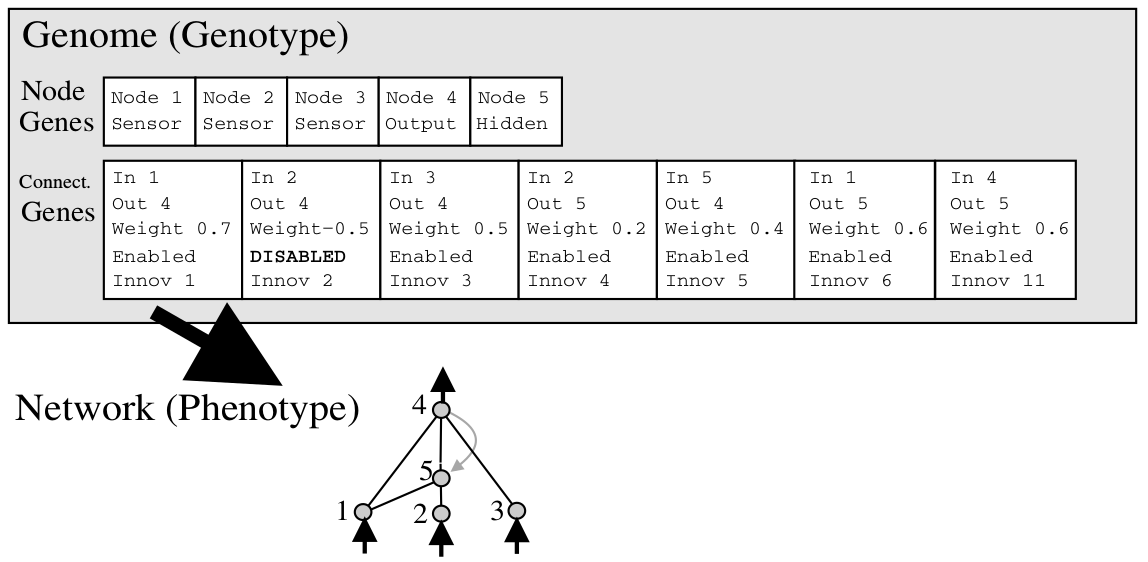
\includegraphics[width=\textwidth]{fig/neat-encoding-example.png}
\caption{Um exemplo de mapeamento entre genótipo e fenótipo de uma rede neural
artificial no \textit{NEAT}. Existem três neurônios (nodos) de entrada, um
escondido e um de saída, e sete conexões (uma recorrente). O segundo gene de
conexão (entre os nodos 2 e 4) está desabilitado, então não é expressado no
fenótipo.}
\label{fig:neat-encoding-example}
\end{figure}

\todo[inline]{Refazer vetorial ou dar autoria 1}


A mutação no \textit{NEAT} modifica os pesos das conexões e as estruturas das
redes. Existe uma chance, a cada geração, de ocorrer uma perturbação nos genes
dos pesos das conexões. As modificações das estruturas das redes -- ilustradas
na Figura \ref{fig:neat-structural-mutation} -- podem ocorrer através da
\textbf{adição de conexões} ou através da \textbf{adição de neurônios}, que
adicionam genes e, consequentemente, expandem o tamanho do genoma. Na adição de
conexões, um gene de conexão é criado com um valor de peso aleatório e passa a
conectar dois neurônios não conectados anteriormente. Na adição de neurônios,
uma conexão existente é desabilitada e um novo neurônio é inserido em seu lugar.
Depois, duas novas conexões são inseridas, e a conexão que leva ao novo neurônio
ganha um peso de valor 1 e a conexão que sai do novo neurônio recebe o mesmo
peso que a conexão desabilitada. Esta forma de adicionar novos neurônios
minimiza o impacto inicial da mutação, pois afeta muito pouco a função da rede.

% NEAT, figure 3
\begin{figure}[H]
\centering
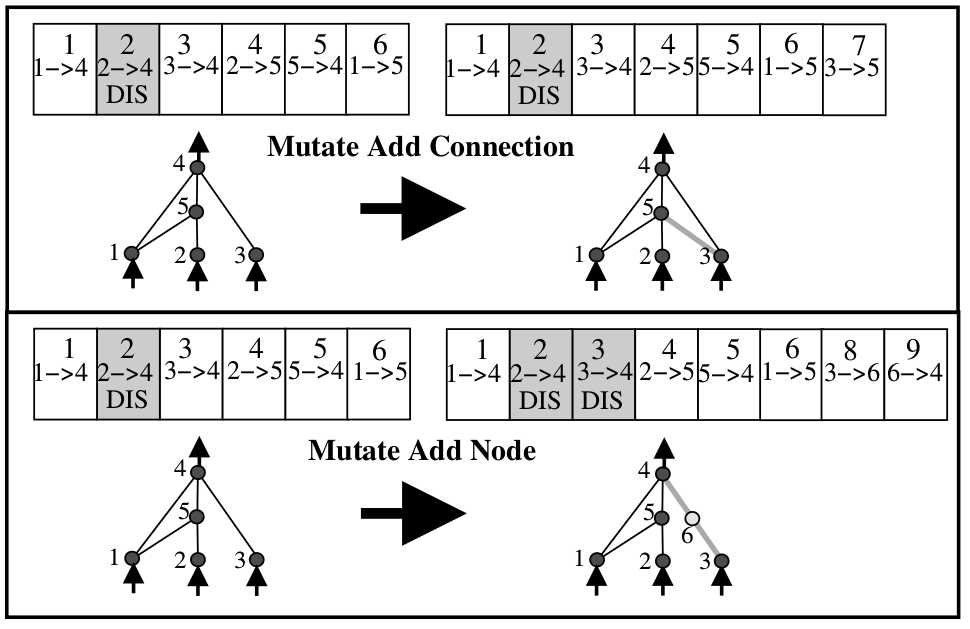
\includegraphics[width=\textwidth]{fig/neat-mutation-examples.png}
\caption{Exemplos das mutações estruturais (adição de conexões e neurônios) que
podem ocorrer no \textit{NEAT}.}
\label{fig:neat-structural-mutation}
\end{figure}

\todo[inline]{Refazer vetorial ou dar autoria 2}

A execução de uma mutação no \textit{NEAT} possui diversas consequências. A
primeira é que os genomas das soluções dos problemas do \textit{NEAT} vão
gradativamente aumentando de tamanho, o que também resulta na aparição de
genomas de tamanhos variados. A segunda consequência é que é possível que surjam
redes que representam a mesma solução mas com codificações genéticas diferentes.
A reprodução destas redesm se não for feita com cautela, pode gerar resultados
ruin, pois pode haver perda de informação. Estas consequências dão origem ao
\textbf{problema da permutação}.

O problema da permutação foi resolvido no \textit{NEAT} da seguinte maneira:
existe uma informação não-explorada na evolução que nos permite dizer exatamente
quais genes de uma população podem ser recombinados. Esta informação é a origem
histórica do gene. Dois genes com a mesma origem histórica devem representar a
mesma estrutura (mesmo que com pesos de conexões diferentes), já que possuem um
ancestral comum. Assim, basta que o sistema saiba as origens históricas dos
genes para garantir mutações de sucesso.  O \textbf{número de inovação} é
responsável por armazenar estas origens históricas.  Toda vez que um gene é
criado através da mutação estrutural, um número global de inovação é
incrementado e o gene recebe seu valor, representando seu ponto de aparecimento
cronológico no sistema.  Durante o processo de recombinação, ilustrado na Figura
\ref{fig:neat-innovation-matchup}, os genes de valores de inovação iguais,
chamados de \textit{matching genes}, são pareados e são escolhidos
aleatóriamente para serem passados adiante. Já os genes que não possuem um par
não podem sofrer mutações, chamados de \textit{disjoint genes} (discontinuidade
no meio da sequência de número de inovação) e \textit{excess genes}
(discontinuidade no fim da sequência de número de inovação), e os genes dos pais
mais aptos são enviados para a prole.

% NEAT, figure 4
\begin{figure}[H]
\centering
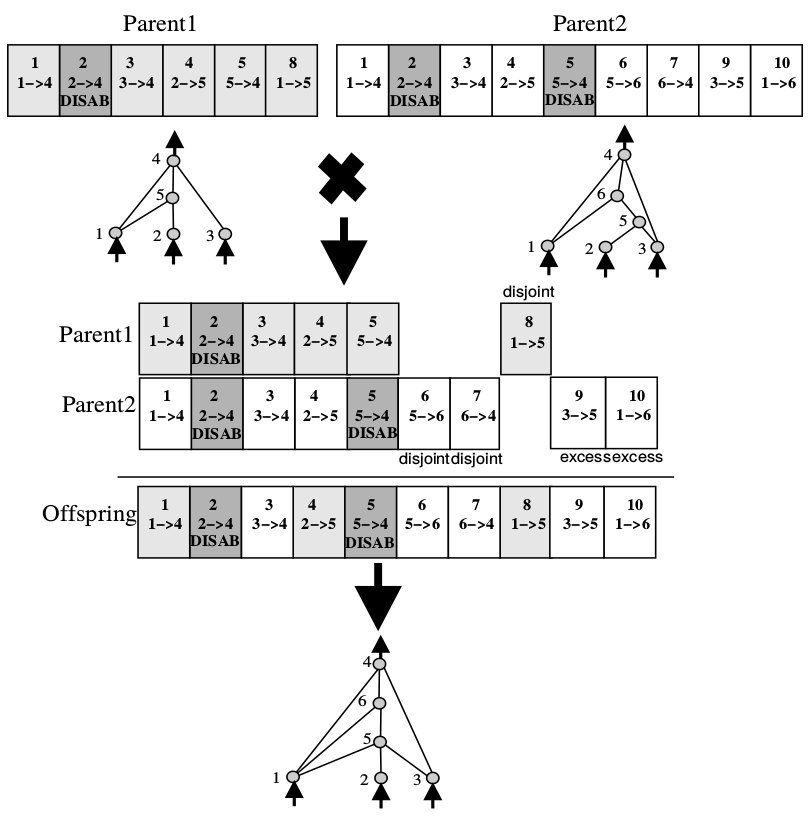
\includegraphics[width=\textwidth]{fig/neat-crossover-example.png}
\caption{Ilustração do alinhamento entre dois genomas de redes neurais
artificiais diferentes. Mesmo que os pais aparentem ser diferentes, seus números
de inovações (mostrado no topo de cada gene) nos informam quais genes serão
herdados. Os \textit{matching genes} são herdados aleatóriamente e os
\textit{disjoint genes} e \textit{excess genes} são herdados do pai com maior
aptidão.}
\label{fig:neat-innovation-matchup}
\end{figure}

\todo[inline]{Refazer vetorial ou dar autoria 3}

Ao adicionar novos genes na população, o sistema é capaz de formar uma população
de topologias diversas. Contudo, devido ao fato de que topologias menores são
otimizadas mais rapidamente que estruturas maiores, a adição de mutações (novos
neurônios e conexões) geralmente traz consigo um decréscimo do valor de aptidão
da rede. Este é o \textbf{problema da proteção da inovação}, que prevê que
estruturas recentemente aumentadas possuem chances pequenas de sobreviver mais
do que uma geração, pois não recebem tempo suficiente para se desenvolver. Para
resolver este problema, o \textit{NEAT} optou por utilizar um sistema de
\textbf{especiação} da população, fazendo com que os indivíduos compitam
principalmente com indivíduos da mesma espécie. Para calcular a diferença
($\delta$) entre dois genomas -- expressada na fórmula \ref{eq:neat-species}
--, é feita uma combinação linear do número de \textit{excess genes} ($E$),
\textit{disjoint genes} ($D$) e a diferença entre a média dos pesos dos
\textit{matching genes} ($\overline{W}$), incluindo genes desabilitados:	

\begin{equation}
\label{eq:neat-species}
\delta = \frac{c_1E}{N} + \frac{c_2D}{N} + c_3\overline{W}
\end{equation}

Os coeficientes $c_1$, $c_2$ e $c_3$ permitem que o desenvolvedor ajuste a
importância dos fatores $E$, $D$ e $\overline{W}$, respectivamente, e o fator
$N$ (número de genes no maior genoma) normaliza a função de acordo com o tamanho
dos genomas. Durante a execução do algoritmo, uma lista ordenada das espécies é
mantida e cada espécie é representada pelo genoma de um de seus membros
(escolhido aleatóriamente) da geração \textbf{passada}. Assim, para classificar
os indivíduos a cada geração, é realizada uma comparação de similaridade entre
os genomas representantes e os genomas a serem categorizados. Se o valor de
similaridade não ultrapassar o limiar de compatibilidade $\delta_t$ (que também
é estabelecido pelo desenvolvedor), o genoma é incluído na espécie. Caso o
genoma não se encaixe em nenhuma espécie, uma nova espécie é criada para ele (e
ele se torna o representante).

Os \textit{TWEANNs} geralmente iniciam com uma população de topologias
aleatórias para introduzir diversidade logo de início. Em contraste, o
\textit{NEAT} inicializa todos os indivíduos de sua população inicial da mesma
maneira: redes com nenhuma camada escondida (ou seja, as entradas se conectam
diretamente com as saídas). Isto faz com que o sistema tenha uma tendência a
procurar por espaços com dimensões reduzidas, pois, quando novas estruturas são
adicionadas através de mutações, somente as modificações úteis para o sistema
(que aumentem a aptidão da rede) sobreviverão. Em outras palavras, todas as
modificações estruturais são justificáveis e a otimização ocorre em menos
dimensões. Isto ajuda a resolver os problemas da escolha de uma
\textbf{população inicial} adequada e da \textbf{inovação topológica} presente
em \textit{TWEANNs} e sistemas de neuroevolução de topologia fixa.


%----------
\section{\label{section:behavior-trees}Behavior Trees}
\todo[inline]{Remover seção sobre Behavior Trees}
A construção de bons agentes inteligentes depende fortemente da capacidade que
os agentes têm de tomar boas decisões de comportamento. No contexto de jogos
digitais, a partir da década de 90, a qualidade da inteligência artificial
passou a ser um diferencial no momento de compra de um jogo\cite[Cap.
1]{Millington:2009:AIG:1795711}, aumentando a importância da escolha de uma
técnica apropriada para desenvolver os agentes inteligentes.Das técnicas mais
populares, a \textbf{\textit{Behavior Tree}}, ou Árvore de Comportamento, é uma
das técnicas que mais se destaca, devido a sua \textbf{simplicidade} e
\textbf{extensibilidade}\cite[Cap.  4]{Rabin:2013:GAP:2566761}, e já foi
utilizada na indústria em jogos como \textit{Halo 2}\cite[Cap.
5]{Millington:2009:AIG:1795711} e
\textit{Spore}\footnote{http://chrishecker.com/My\_liner\_notes\_for\_spore},
por exemplo.

Uma \textit{Behavior Tree} é uma estrutura de dados baseada em árvore que contém
um nodo \textbf{raíz} (geralmente utilizada para controlar o fluxo inicial de
execução) e vários nodos filhos que representam os \textbf{comportamentos}. Cada
comportamento deve possuir uma \textbf{pré-condição} e uma \textbf{ação}. Caso a
pré-condição seja satisfeita, o agente poderá executar o comportamento descrito
pela ação do nodo\cite[Cap. 4]{Rabin:2013:GAP:2566761}. Isto faz com que o
algoritmo de execução seja simples: partimos do nodo raíz em busca do primeiro
filho que satisfaça sua pré-condição (geralmente da esquerda para a direita). Ao
encontrá-lo, executamos sua ação. É importante ressaltar que somente um
comportamento é selecionado por vez. Portanto, se um comportamento for
selecionado, o algoritmo não tentará executar as ações dos nodos vizinhos na
mesma execução do algoritmo.

É possível adicionar estruturas de \textbf{controle de fluxo} a uma
\textit{Behavior Tree}. Desta forma, os ramos da árvore passam a ser usados para
controlar o fluxo de execução, enquanto os nodos-folha representam as
pré-condições e ações\cite[Cap. 10]{Rabin:2015:GAP:2821138}. Quando uma ação de
um nodo-folha é executado, ele informa ao seu pai (controlador de fluxo) o
estado de sua execução -- sucesso, falha ou em andamento. Existem diversos
tipos de estruturas de controle de fluxo que são utilizadas em \textit{Behavior
Trees}, mas as mais comuns são os de \textbf{seleção} e de \textbf{sequência}.

O algoritmo do controle de fluxo de seleção -- exemplificado no algoritmo
\ref{alg:behavior-tree-selection} -- faz a execução do \textbf{primeiro nodo
filho} que tiver sua pré-condição satisfeita. Quando termina de executar a ação
selecionada, aborta o procedimento, não visitando as demais ações.
Diferentemente do algoritmo de seleção, o algoritmo de \textbf{sequência} --
exemplificado no algoritmo \ref{alg:behavior-tree-sequence} -- tentará executar
\textbf{todos} os nodos que satisfizerem suas pré-condições de forma
\textbf{sequencial}. Sua execução só é interrompida quando não for possível
tomar a ação descrita pelo nodo ou quando não existirem mais nodos para se
avaliar.

\begin{algorithm}[H]
\begin{center}
	% Um exemplo de algoritmo utilizando a pacote 'algorithmic'
	%\algsetup{linenosize=\small,linenodelimiter=.}
	\begin{algorithmic}[1]
        \STATE filhos $\gets$ lista de nodos filhos
        \FOR{cada filho em filhos}
            \IF{filho.executar() == true}
                \RETURN true
            \ENDIF
        \ENDFOR
        \RETURN false
    \end{algorithmic}
\end{center}
\caption[Algoritmo para execução do controle de fluxo do tipo seleção em uma
behavior tree.]
{\label{alg:behavior-tree-selection} Algoritmo para execução do controle de
fluxo do tipo seleção em uma behavior tree.}
\end{algorithm}

\begin{algorithm}[H]
\begin{center}
	% Um exemplo de algoritmo utilizando a pacote 'algorithmic'
	%\algsetup{linenosize=\small,linenodelimiter=.}
	\begin{algorithmic}[1]
        \STATE filhos $\gets$ lista de nodos filhos
        \FOR{cada filho em filhos}
            \IF{filho.executar() == false}
                \RETURN false
            \ENDIF
        \ENDFOR
        \RETURN true
    \end{algorithmic}
\end{center}
\caption[Algoritmo para execução do controle de fluxo do tipo sequência em uma
behavior tree.]
{\label{alg:behavior-tree-sequence} Algoritmo para execução do controle de fluxo
do tipo sequência em uma behavior tree.}
\end{algorithm}

Para que fique mais claro como a técnica é utilizada, criamos um cenário
hipotético onde devemos criar a inteligência artificial de um agente (um robô
doméstico) que tem uma tarefa muito importante: limpar e organizar os móveis da
sala de estar de uma casa. Este robô, contudo, é movido à baterias, que não
duram muito. Então, de tempos em tempos, é necessário que ele recarregue suas
energias. Existem duas fontes de energia disponíveis para o robô: energia solar
e energia elétrica. A energia solar é preferível, por ser uma forma de energia
mais limpa, mas nem sempre é possível utilizá-la (um dia chuvoso, por exemplo).
Caso o robô termine suas tarefas e não esteja com níveis baixos de bateria, pode
descansar, entrando em modo de repouso.  A Figura
\ref{fig:behavior-tree-example} representa o comportamento deste agente através
de uma \textit{Behavior Tree}. Para decidir entre as fontes de energia, usamos
um controle de fluxo do tipo \textbf{seleção}, pois somente um tipo de energia
deve ser utilizado. Já para executar suas tarefas (limpar e organizar), usamos
um controle de fluxo do tipo \textbf{sequência}, pois todas as tarefas devem ser
executadas.

\begin{figure}[H]
\centering
\begin{tikzpicture}[
    every node/.style={
        font=\scriptsize
    },
    composite/.style={
        minimum width=1.3cm, minimum height=1.2cm,
        text width=1.3cm,
        text centered,
        rounded rectangle,
        draw
    },
    action/.style={
        minimum width=1.3cm, minimum height=1.2cm,
        text width=1.3cm,
        text centered,
        rectangle,
        draw
    },
    precond/.style={
        minimum width=1.3cm, minimum height=1.2cm,
        text width=1.3cm,
        text centered,
        rectangle,
        fill=black,
        text=white
    }
]
\matrix [row sep=1cm, column sep=0.3cm] {
                                                &
                                                &
                                                &
    \node (n1)  [action]    {Raíz};             &
                                                &
                                                &
                                                &
                                                &
                                                &
    \\
                                                &
    \node (n2)  [composite] {Selecionar};       &
                                                &
                                                &
    \node (n4)  [composite] {Sequência};        &
                                                &
    \node (n3)  [action]    {Descansar};        &
                                                &
                                                &
    \\
    \node (n5)  [precond]   {Pouca Energia?};   &
    \node (n7)  [action]    {Energia Solar};    &
    \node (n6)  [action]    {Energia Elétrica}; &
    \node (n8)  [precond]   {Casa Suja?};       &
    \node (n9)  [action]    {Limpar Sala};      &
    \node (n10) [action]    {Organizar Móveis}; &
                                                &
                                                &
                                                &
    \\
};
\draw[->,>=latex] (n1.south) -- (n2.north);
\draw[->,>=latex] (n1.south) -- (n3.north);
\draw[->,>=latex] (n1.south) -- (n4.north);

\draw[->,>=latex] (n2.south) -- (n5.north);
\draw[->,>=latex] (n2.south) -- (n6.north);
\draw[->,>=latex] (n2.south) -- (n7.north);

\draw[->,>=latex] (n4.south) -- (n8.north);
\draw[->,>=latex] (n4.south) -- (n9.north);
\draw[->,>=latex] (n4.south) -- (n10.north);
\end{tikzpicture}
\caption {\label{fig:behavior-tree-example}Exemplo de uma \textit{behaviour
tree} para representar um agente que deve carregar suas baterias caso seja
necessário, além de limpar e organizar a casa, descansando caso contrário. Os
retângulos brancos, pretos e arredondados representam, respectivamente, as
ações, as pré-condições e os controles de fluxo.}
\end{figure}

Existem algumas outras técnicas que resolvem o mesmo problema que as
\textit{Behavior Trees} e são muito utilizadas em inteligência artificial para
jogos como, por exemplo, as \textbf{\textit{Finite State Machines}} (máquinas de
estados finitos) e as \textbf{\textit{Hierarchical Finite State Machines}}
(máquinas de estados finitos hierárquicos). As \textit{FSMs} contém
\textbf{estados} que são ligados através de \textbf{transições}. Existem
diversos problemas com esta abordagem, como o crescimento exponencial de estados
e transições, a impossibilidade de fácil reutilização dos estados e a possível
existência de transições inválidas no modelo. As \textit{FSMs} possuem,
resumidamente, um problema de modularidade. As \textit{HFSMs} surgiram
justamente para mitigar alguns dos problemas presentes nas \textit{FSMs},
permitindo o englobamento de estados em uma hierarquia. Entretanto, o problema
de extensibilidade e praticidade ainda existem, porque ainda é baseada em
transições.
